\documentclass[professionalfonts]{beamer}
\usepackage[familydefault,light]{Chivo} 
\usepackage[T1]{fontenc}
\usenavigationsymbolstemplate{}
\usepackage[]{hyperref}
\usepackage{tikz,pgf,pgfarrows,pgfnodes,pgfbaseimage}
\graphicspath{{./Pics/}}
\usetikzlibrary{shapes}
\usepackage{setspace}
\newcommand{\evi}[1]{{\colorbox{yellow!50}{{#1}}}}
\newcommand{\exe}[1]{{\color{black!50}{{#1}}}}
\newcommand{\kw}[1]{{\colorbox{black!30}{\color{white}{#1}}}}
\tikzstyle{nd}=[circle,draw=black,thick,minimum size=.8cm,inner sep=1pt]
\setbeamercovered{transparent}
\usetheme{Singapore}
\tikzstyle{nodo}=[ellipse,draw=black!60,fill=black!10,line width=.7pt,minimum width=.7cm,minimum height=.4cm]
\usecolortheme[named=gray]{structure}
\setbeamercolor{block title}{bg=black!20,fg=black}
\setbeamercolor{block body}{bg=black!10,fg=black}

\title{Algoritmi Numerici (Parte II)}
\subtitle{[Lezione 2] Algoritmo della secante e della tangente}
\author{Alessandro Antonucci\\{\tt alessandro.antonucci@supsi.ch}}
\date{\tiny\url{https://colab.research.google.com/drive/1Iv2YA4iBL8g54yY1bdcRgtFNqI4LF7Kw}}
%%%%%%%%%%%%%%%%%%%%%%%%%%%%
\begin{document}
\maketitle
\setstretch{1.4}
\frame{\frametitle{Ricorsioni}
\begin{itemize}
\item Sequenza $x_0$, $x_1$, $x_2$, $\ldots$ generata da una ricorsione
\item (ex1) fattoriale $x_{j+1} = (j+1) x_j$ (con $x_0=1$)
\item (ex2) Fibonacci $x_{j+1} = x_j + x_{j-1}$ (con $x_0=1$ e $x_1=2$)
\item ex1 ricorsione ordine 1,\\inizializzazione solo del primo elemento
\item ex2 ricorsione ordine 2,\\inizializzazione dei primi due elementi
\end{itemize}}



\frame{\frametitle{Identificazione degli zeri mediante sequenze}
\begin{itemize}
\item Approssimare zero $x^*$ di una funzione $f(x)$?
\item Sequenza $x_0$, $x_1$, $\ldots$, $x_n$ che si avvicina ad $x^*$
\item Convergenza: $\lim_{n\to+\infty} |x_n-x^*| = 0$
\end{itemize}
\begin{columns}
\begin{column}[T]{0.5\textwidth}
\begin{block}{SECANTE}
\begin{center}
$x_{j+1} = x_j - \frac{f(x_j)}{ \frac{f(x_j)-f(x_{j-1})}{x_j-x_{j-1}}}$
\end{center}
\end{block}
\end{column}
\begin{column}[T]{0.5\textwidth}
\begin{block}{TANGENTE}
\begin{center}
$x_{j+1} = x_j - \frac{f(x_j)}{f'(x_j)}$
\end{center}
\end{block}
\end{column}
\end{columns}
\begin{center}
\emph{Nota: nessuno dei due algoritmi da' garanzie di convergenza}
\end{center}}


\frame{\frametitle{Algoritmo della Secante}
\setbeamercovered{}
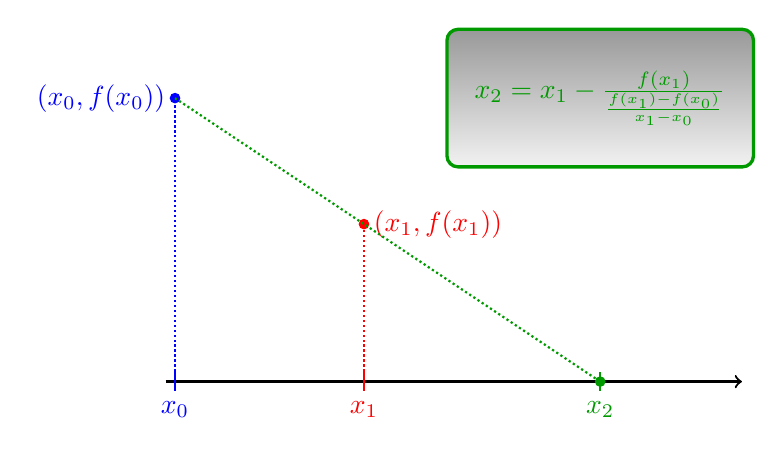
\begin{tikzpicture}[domain=0:3.5,scale=1.2]
\draw[->,thick] (-.1,0) -- (6,0);
\draw[thick,color=orange] plot[id=exp] function{3-x*x*1/3}; 
\pause
\draw[blue,thick] (0,.1) -- (0,-.1) node[below] {$x_0$};
\draw[red,thick] (2,.1) -- (2,-.1) node[below] {$x_1$};
\pause
\draw[blue,densely dotted,thick] (0,0) -- (0,3);
\draw [blue,fill] (0,3) circle [radius=0.05] node[left] {$(x_0,f(x_0))$};
\draw [red,fill] (2,5/3) circle [radius=0.05] node[right] {$(x_1,f(x_1))$};
\draw[densely dotted,red,thick] (2,0) -- (2,5/3);
\pause
\draw[densely dotted,green!60!black,thick] (0,3) -- (9/2,0);
\pause
\draw [green!60!black,fill] (9/2,0) circle [radius=0.05] node[right] {};
\draw[green!60!black,thick] (9/2,.1) -- (9/2,-.1) node[below] {$x_2$};
\draw[green!60!black,thick] (9/2,3) node[top color=black!40,bottom color=black!5,very thick,draw,rectangle, rounded corners, inner sep=10pt, inner ysep=15pt] {$x_2=x_1-\frac{f(x_1)}{\frac{f(x_1)-f(x_0)}{x_1-x_0}}$};
\end{tikzpicture}}


\frame{\frametitle{Algoritmo della Tangente}
\setbeamercovered{}
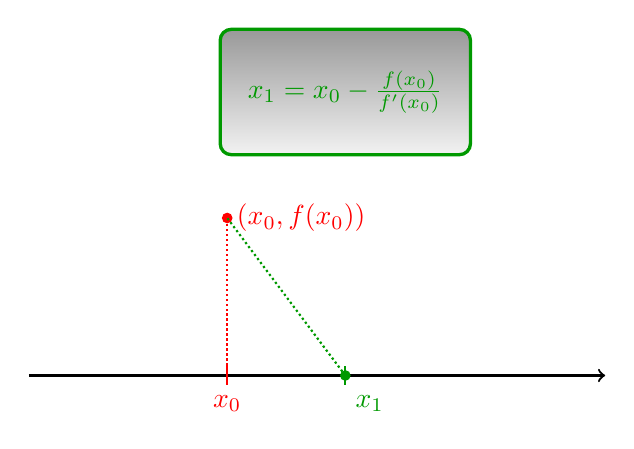
\begin{tikzpicture}[domain=0:3.5,scale=1.2]
\draw[->,thick] (-.1,0) -- (6,0);
\draw[thick,color=orange] plot[id=exp] function{3-x*x*1/3}; 
\pause
\draw[red,thick] (2,.1) -- (2,-.1) node[below] {$x_0$};
\pause
\draw [red,fill] (2,5/3) circle [radius=0.05] node[right] {$(x_0,f(x_0))$};
\draw[densely dotted,red,thick] (2,0) -- (2,5/3);
\pause
\draw[densely dotted,green!60!black,thick] (13/4,0) -- (2,5/3);
\pause
\draw [green!60!black,fill] (13/4,0) circle [radius=0.05] node[right] {};
\draw[green!60!black,thick] (13/4,.1) -- (13/4,-.1) node[below right] {$x_1$};
\draw[green!60!black,thick] (13/4,3) node[top color=black!40,bottom color=black!5,very thick,draw,rectangle, rounded corners, inner sep=10pt, inner ysep=15pt] {$x_1=x_0-\frac{f(x_0)}{f'(x_0)}$};
\end{tikzpicture}}







\frame{\frametitle{Algoritmo della Secante}
\setbeamercovered{}
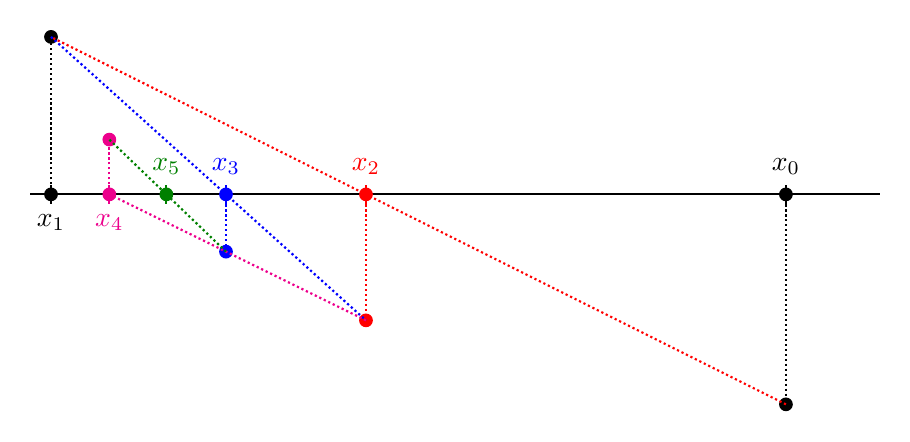
\begin{tikzpicture}[domain=0.5:3.3,scale=4]
\draw[-,thick] (0.6,0) -- (3.3,0);
\draw[thick,color=black] plot[id=exp] function{1/x-1}; 
\pause
\draw[black,thick] (3,-.03) -- (3,.03) node[above] {$x_0$};
\draw[black,thick] (2/3,.03) -- (2/3,-.03) node[below] {$x_1$};
\draw [black,fill] (3,0) circle [radius=0.02] node[left] {};
\draw [black,fill] (2/3,0) circle [radius=0.02] node[right] {};
\pause
\draw[black,densely dotted,thick] (3,0) -- (3,-2/3);
\draw[black,densely dotted,thick] (2/3,0) -- (2/3,1/2);
\draw [black,fill] (3,-2/3) circle [radius=0.02] node[left] {};
\draw [black,fill] (2/3,1/2) circle [radius=0.02] node[right] {};
\pause
\draw[densely dotted,thick,red] (3,-2/3) -- (2/3,1/2);
\pause
\draw [red,fill] (5/3,0) circle [radius=0.02] node[right] {};
\draw[red,thick] (5/3,-.03) -- (5/3,.03) node[above] {$x_2$};
\pause
\draw[densely dotted,thick,red] (5/3,0) -- (5/3,-2/5);
\draw [red,fill] (5/3,-2/5) circle [radius=0.02] node[right] {};
\pause
\draw[densely dotted,thick,blue] (2/3,1/2) -- (5/3,-2/5);
\pause
\draw [blue,fill] (11/9,0) circle [radius=0.02] node[right] {};
\draw[blue,thick] (11/9,-.03) -- (11/9,.03) node[above] {$x_3$};
\pause
\draw[densely dotted,thick,blue] (11/9,0) -- (11/9,-2/11);
\draw [blue,fill] (11/9,-2/11) circle [radius=0.02] node[right] {};
\pause
\draw[densely dotted,thick,magenta] (5/3,-2/5) -- (23/27,0);
\pause
\draw [magenta,fill] (23/27,0) circle [radius=0.02] node[right] {};
\draw[magenta,thick] (23/27,.03) -- (23/27,-.03) node[below] {$x_4$};
\pause
\draw[densely dotted,thick,magenta] (23/27,0) -- (23/27,4/23);
\draw [magenta,fill] (23/27,4/23) circle [radius=0.02] node[right] {};
\pause
\draw[densely dotted,thick,green!50!black] (11/9,-2/11) -- (23/27,4/23);
\pause
\draw [green!50!black,fill] (251/243,0) circle [radius=0.02] node[right] {};
\draw[green!50!black,thick] (251/243,-.03) -- (251/243,.03) node[above] {$x_5$};
\end{tikzpicture}}
\end{document}
\frame{\frametitle{Interpretazione grafica}
\begin{columns}
\begin{column}[T]{0.5\textwidth}
TANGENTE
\end{column}
\begin{column}[T]{0.5\textwidth}
SECANTE
\end{column}
\end{columns}
\includegraphics[width=10cm]{PicsAndStyle/s.png}
}

\end{document}

		\vskip 1mm \`e possibile usare una relazione ricorsiva
\item Es. il fattoriale \`e una ricorsione di ordine 1: $x_{n+1} = (n+1) x_n$, con $x_0=1$
\item Es. Fibonacci \`e una ricorsione di ordine 2: $x_{n+1} = x_n + x_{n_1}$, con $x_0=1$, $x_1=2$
\item Nota: ricorsione di ordine 1, ha bisogno di inizializzare un elemento
	ricorsione di ordine 2, richiede inizializzazione dei primi due termini
\end{itemize}}





\end{document}
%%%%%%%%%%%%%%%%%%%%%%%%%%%%
\frame{\frametitle{La bisezione}
\begin{itemize}
\item Dopo aver localizzato $x^*$ sull'intervallo $[a,b]$
\item Prendo il punto medio $c:=\frac{a+b}{2}$
\item La funzione cambia segno su $[a,c]$ \evi{oppure} su $[c,b]$
\item Nel primo caso $x^*\in[a,c]$, \\ nel secondo $x^*\in [c,b]$
\end{itemize}
\begin{center}
\color{black!50}{In entrambi i casi, il nuovo intervallo \`e la met\`a del vecchio}
\end{center}}
%%%%%%%%%%%%%%%%%%%%%%%%%%%%
\frame{\frametitle{La bisezione (pseudo codice)}
\begin{columns}
\begin{column}[T]{0.4\textwidth}
\tt
if f(a)*f(b)< 0 \\
\quad for k = 1:n, \\      
\quad\quad	c = (a+b)/2;  \\  	
\quad\quad	if f(a)*f(c) < 0	\\
\quad\quad\quad b = c; \\     
\quad\quad else\\
\quad\quad\quad a = c;\\
\quad\quad end\\
\quad end\\
end
\end{column}
\begin{column}[T]{0.4\textwidth}
\begin{center}
L'algoritmo
pu\`o essere 
iterato
ricorsivamente\\
{\tt n} volte
\vskip 2mm
\evi{Criteri d'arresto} alternativi\\
{\tt while errmax > eps}\\
oppure\\
{\tt while |f(c)| > eps}\\
\end{center}
\end{column}
\end{columns}}
%%%%%%%%%%%%%%%%%%%%%%%%%%%%

\frame{\frametitle{Analisi precisione}
\begin{itemize}
\item Intervallo iniziale $[a^0,b^0]$, stima puntuale $c^0:=\frac{a^0+b^0}{2}$
\item $x^* \in [a^0,b^0]$ e $\epsilon^0:=|x^*-c^0|< \frac{b^0-a^0}{2}$
\item Analogamente, $\epsilon^k < \frac{b^0-a^0}{2^{k+1}}$
\end{itemize}
\begin{center}
\color{black!50}{Con la bisezione posso quindi prevedere\\quante iterazioni servono per rendere l'errore minore\\di un valore prefissato}
\end{center}}

\frame{\frametitle{Osservazione}
\begin{itemize}
\item L'algoritmo di bisezione si basa sulla scelta di un punto $c$ interno all'intevallo $[a,b]$
\item Scegliere il punto medio ha il vantaggio/svantaggio di rendere il nuovo intervallo la met\`a di quello vecchio
\item Ogni altra scelta di $c\in[a,b]$ permette comunque di procedere
\item In particolare, nella scelta di $c$ pu\`o essere utile considerare il valore (e non solo il segno) della
	funzione in $f(a)$ e $f(b)$
\end{itemize}
}

\frame{\frametitle{Regula Falsi}
\begin{itemize}
\item Variante dell'algoritmo di bisezione 
\item $c$ \`e il punto d'incontro con l'asse $x$ della retta che passa per i punti di coordinate $(a,f(a))$ e $(b,f(b))$
\end{itemize}
\vskip 2mm
$$c:= a - \frac{f(a)}{\frac{f(b)-f(a)}{b-a}}$$}

\frame{\frametitle{Regula Falsi (ii)}
\begin{itemize}
\item Tipicamente, dopo un certo numero di iterazioni, la regula falsi sposta sempre l'estremo destro (o sempre quello sinistro) dell'intervallo
\item Se sull'intervallo la funzione \`e sempre concava (o convessa), la retta che congiunge i due punti estremi \`e sempre a sx (o sempre a dx) dello zero della funzione
\item In pratica, la regula falsi non si usa mai da sola, ma sempre in congiunzione con altri algoritmi
\end{itemize}}








\end{document}

\begin{verbatim}
if f(a)*f(b)<0,		% Check preliminare
	c = (a+b)/2	% Punto medio
	if f(a)*f(c)<0	% se cambia segno in [a,c]
		b = c	% sposto a sx l'estremo ddx
	else
		a = c	% sposto a dx l'estremo sx
\end{verbatim}



\frame{\frametitle{Sottrazione (e precisione multipla)}
\begin{itemize}
\item Somma di due numeri a 4 bit:
\begin{itemize}
\item Due addendi (4+4 bit) 
\item Carry (C, 1 bit) si attiva per il riporto \exe{$1+1=1$ \`e AND}
\item Overflow (V, 1 bit) si attiva per identificare over/under
\end{itemize}
\item Numeri piu grandi
\begin{itemize}
\item Precisione multipla (tante locazioni affiancate)
\item Si inizializza $C=0$ (non importa se alla fine $C=1$)
\item Risultato corretto solo se $V=0$
\end{itemize}
\item Sottrazione
\begin{itemize}
\item a - b = a + (-b)
\item Per scrivere $-b$, scrivo $b$ in base 2 e poi cambio segno \\ (ricopio da dx finch\'e non trovo $1$, scrivo quello, poi nego)
\end{itemize}
\end{itemize}}


\frame{\frametitle{Moltiplicazione e Divisione}
\begin{itemize}
	\item Moltiplicazioni in colonna = somme di numeri spostati a sx
	\item ASL (arithmetic shift left) sposto i bit a sx (uno zero a dx)
	\item Es. ASR(0011)=0110 
	\item \`E moltiplicazione per 2 (se $V=0$ vale anche con complemento a 2)
	\item Divisione: analoga ma sposto a dx
	\item ASR (arithmetic shift right), divisione (intera) per 2
\end{itemize}}

\frame{\frametitle{Aritmetica float}
\begin{itemize}
\item Dati due numeri (float)
\begin{itemize}
\item $a = m_1 \cdot b^q$ 
\item	$b = m_2 \cdot b^p$ ($q>p$)
\end{itemize}
\item Posso calcolare
\begin{itemize}
\item $a+b = (m_1 + m_2 \cdot b^{p-q}) \cdot b^q$
\item $a \cdot b = (m_1 \cdot m_2) \cdot b^{q+p}$
\item $a / b= (m_1 / m_2) \cdot b^{q-p}$
\end{itemize}
\item Le operazioni sulla mantissa introducono un errore\\
(riducono le cifre significative)
\end{itemize}
}


\frame{\frametitle{Under/over flow con numeri float} 
Formati float-like caratterizzati da:
\begin{itemize}
\item $m_1$ numero pi\`u piccolo rappresentabile
\item $M_1$ numero pi\`u grande.
\end{itemize}
Quando inserisco un numero $x$, il sistema restituisce
\begin{itemize}
\item overflow se $x$ esterno a $[-M_1,M_1]$
\item underflow se interno a $(-m_1,m_1)$ (approssimato con lo zero)
\end{itemize}
Nel formato float, se tutti i bit dell'esponente sono uno, casi speciali
\vskip 2mm
Es. $0|11111111|00000000000000000000000\to + \infty$
Es. $0|11111111| 00000000001000001000000 \to NaN$
}


\end{document}
